\chapter{はじめに}
\label{chapter: introduction}

\section{問題設定}
\label{section: problemDefinition}
所与の領域を一人または複数の巡査が動き回り,
その領域内の指定された場所を十分な頻度で訪れることを
警邏(patrolling)という\cite{
  Dumitrescu:2014:CGC:2636805.2636822,
  chen2013fence,
  coene2011charlemagne,
  czyzowicz2011boundary}.
\ncomment{[文献追加]}

本稿では,与えられた距離空間$U$内を巡査$m$人が速さ$1$以下で動きまわることにより,
有限集合$V \subseteq U$に属する点を十分な頻度で訪れるという目標を考える.
距離空間$U$といっても,
$V$の点どうしを結ぶ最短路以外を巡査が歩むことは無駄であるから,
$V$を頂点集合とし,辺に長さのついたグラフを考え,
$U$はその頂点および辺上の点のみからなるとしてよい.
このような空間と点集合の組$(U, V)$を\defword{地図}と呼ぶ.

地図$(U, V)$における
巡査$i \in \{1, \ldots, m\}$の\defword{運行}$a _i \colon \Rset \to U$とは,
各時刻$t \in \Rset$における位置$a _i (t) \in U$を定める函数であって,
移動の速さが$1$以下であるもの,すなわち
任意の時刻$s$,$t \in \Rset$に対し$a _i (s)$と$a _i (t)$の距離が$\abs{s - t}$を超えないものをいう.
巡査$m$人による\defword{運行}とは,
全巡査の運行を定めた組$A = (a _1, \dots, a _m)$をいう.
$V$の各頂点には利得および{\maxIdletime}と呼ばれる正整数が定まっている.
点$v \in V$の{\maxIdletime}が$q$であるとき,
巡査達が運行$A = (a _1, \dots, a _m)$で点$v$を\defword{警邏}するとは,
長さ$q$のどの時間にも
いずれかの巡査が$v$を少なくとも一度は訪れる
(任意の時刻$t \in \Rset$に対して
巡査$i$と時刻$\tau \in [t, t + q)$が存在し$a _i (\tau) = v$)
ことをいう.
巡査達が運行$A$により点集合$W \subseteq V$を\defword{警邏}するとは,
各点$v \in W$に対し巡査達が運行$A$で$v$を警邏することをいう.
そのような運行が存在するとき$W$は$m$人により\defword{警邏可能}であるという.

\begin{patrollingProblem}
  巡査の人数$m \in \Nset$と地図$(U, V)$および
  その各頂点の利得と{\maxIdletime}が与えられる.
  $m$人の巡査により警邏可能な頂点集合のうち
  利得の和が最大となるものを求めよ.
\end{patrollingProblem}

一つの点を複数の巡査の訪問により警邏し得ることに注意されたい.
例えば図\ref{figure: cooperative}左はそのような運行の例である.
\begin{figure}
  \centering
  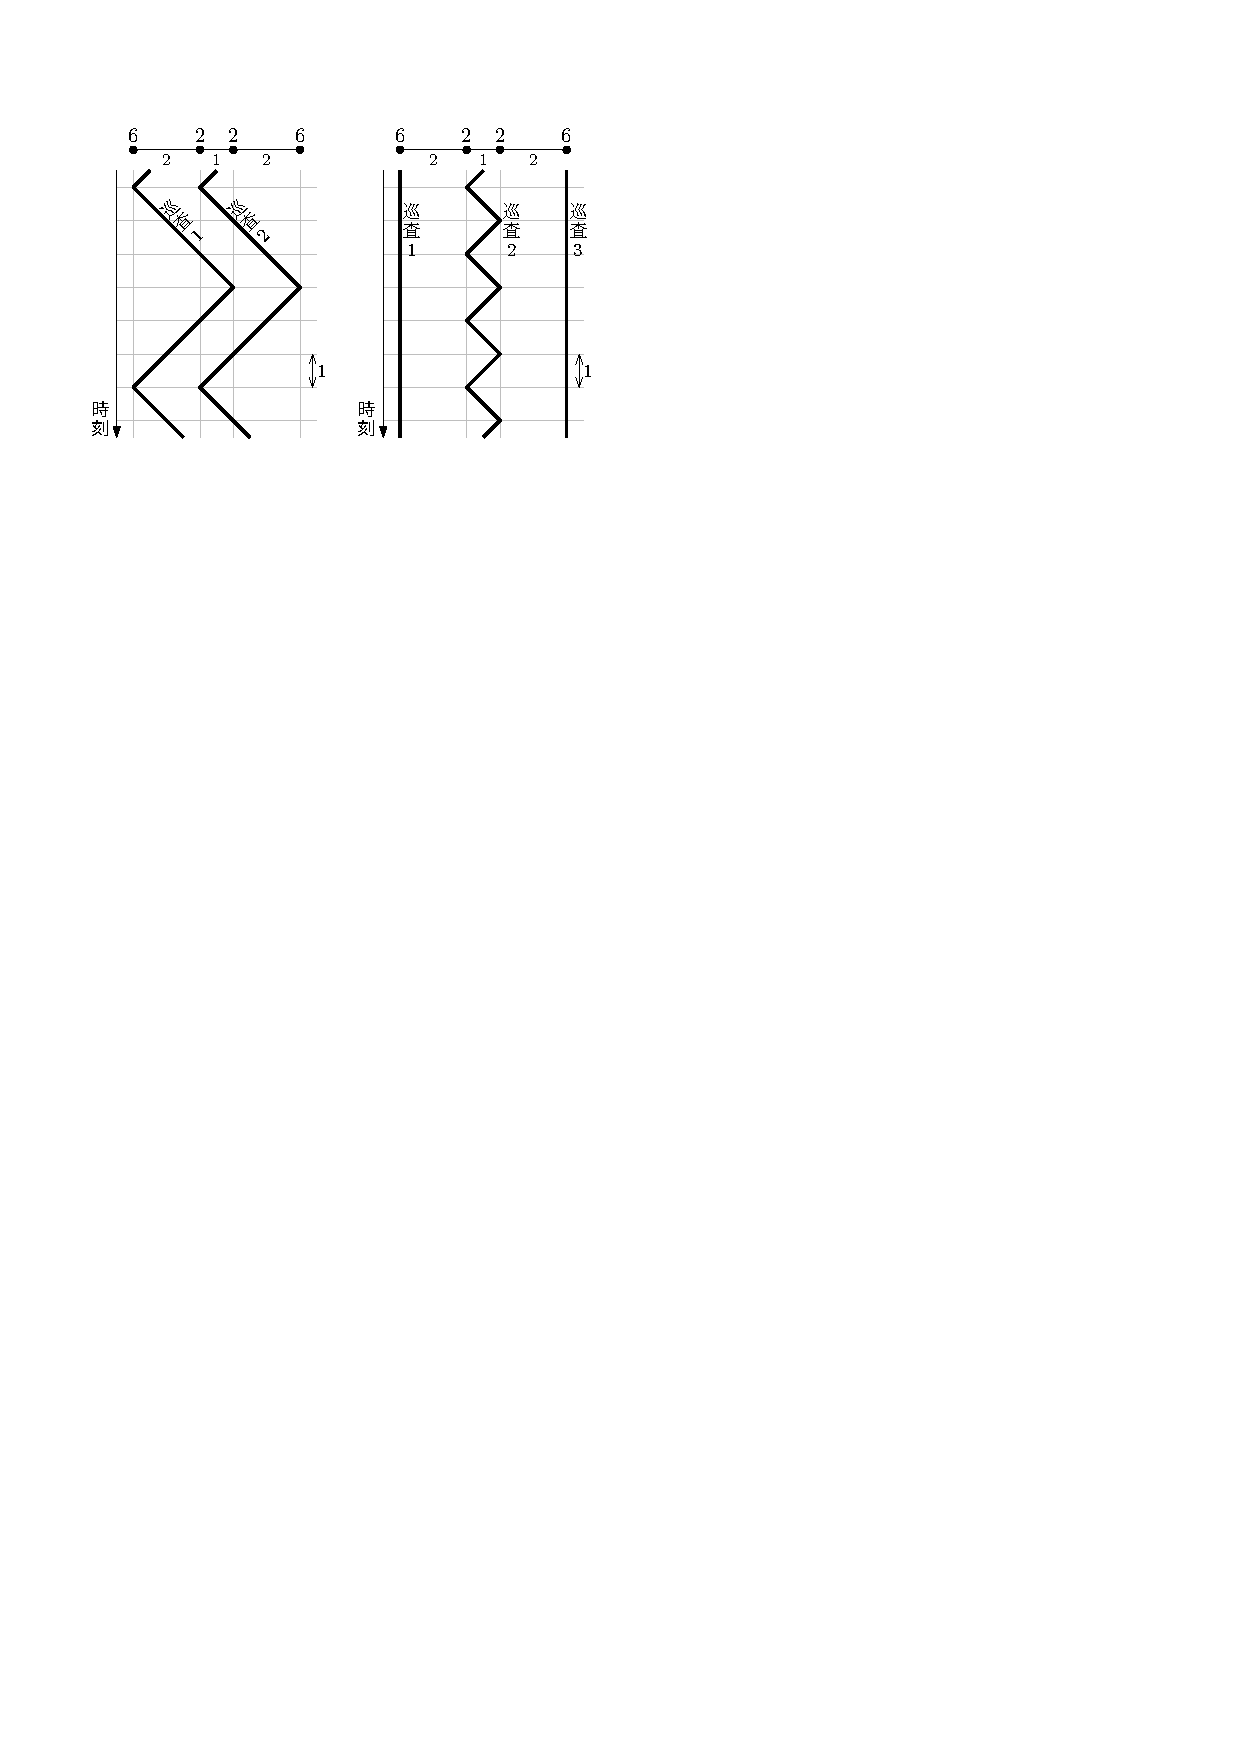
\includegraphics[scale=1.0]{\figdir/cooperative.pdf}
  \caption{図の上部に描かれている四点からなる{\graphLine}の地図の全点を警邏する二つの運行.
    点と辺に書かれた数は,それぞれ{\maxIdletime}と距離である.
    左図の運行では二人の巡査が協力して中央の二点を警邏している.
    これを禁じ,各点がいずれかの巡査により単独警邏されることを求める場合は,
    右図のように三人の巡査を要する.}
  \label{figure: cooperative}
\end{figure}
Coeneら\cite{coene2011charlemagne}は似た問題を扱っているが,
このような協力を許さず,
図\ref{figure: cooperative}右のように
各点を専ら一人の巡査が「担当」することを要求している.
つまり,各点$v \in W$が\defword{単独警邏}される(すなわち
或る一人の巡査がおり,
その巡査のみの運行が$v$を警邏する)ことを要求しているのである.
対比のため本稿ではこの問題を\defword{\independentPatProb}と呼ぶことにする
(\cite{coene2011charlemagne}ではMPLPPと称している).
Coeneら\cite{coene2011charlemagne}の諸結果においては,
この単独警邏という限定が,
多項式時間算法の設計にも困難性の証明にも重要な役割を果している.
この限定を外したときの様子を調べるのが本稿の目的である.

{\patProb}は,巡査が一人かつ
全点の利得と{\maxIdletime}が等しい場合に限っても,
ハミルトン路問題からの帰着により
NP困難である\cite[Theorem~8]{coene2011charlemagne}.
そこで本稿では入力される地図を限定する.
具体的には線分({\graphLine}),星({\graphStar}),
すべての辺の長さが等しい完全グラフ({\graphUnit})を扱う
(図\ref{figure: graph_classes}).
\begin{figure}
  \centering
  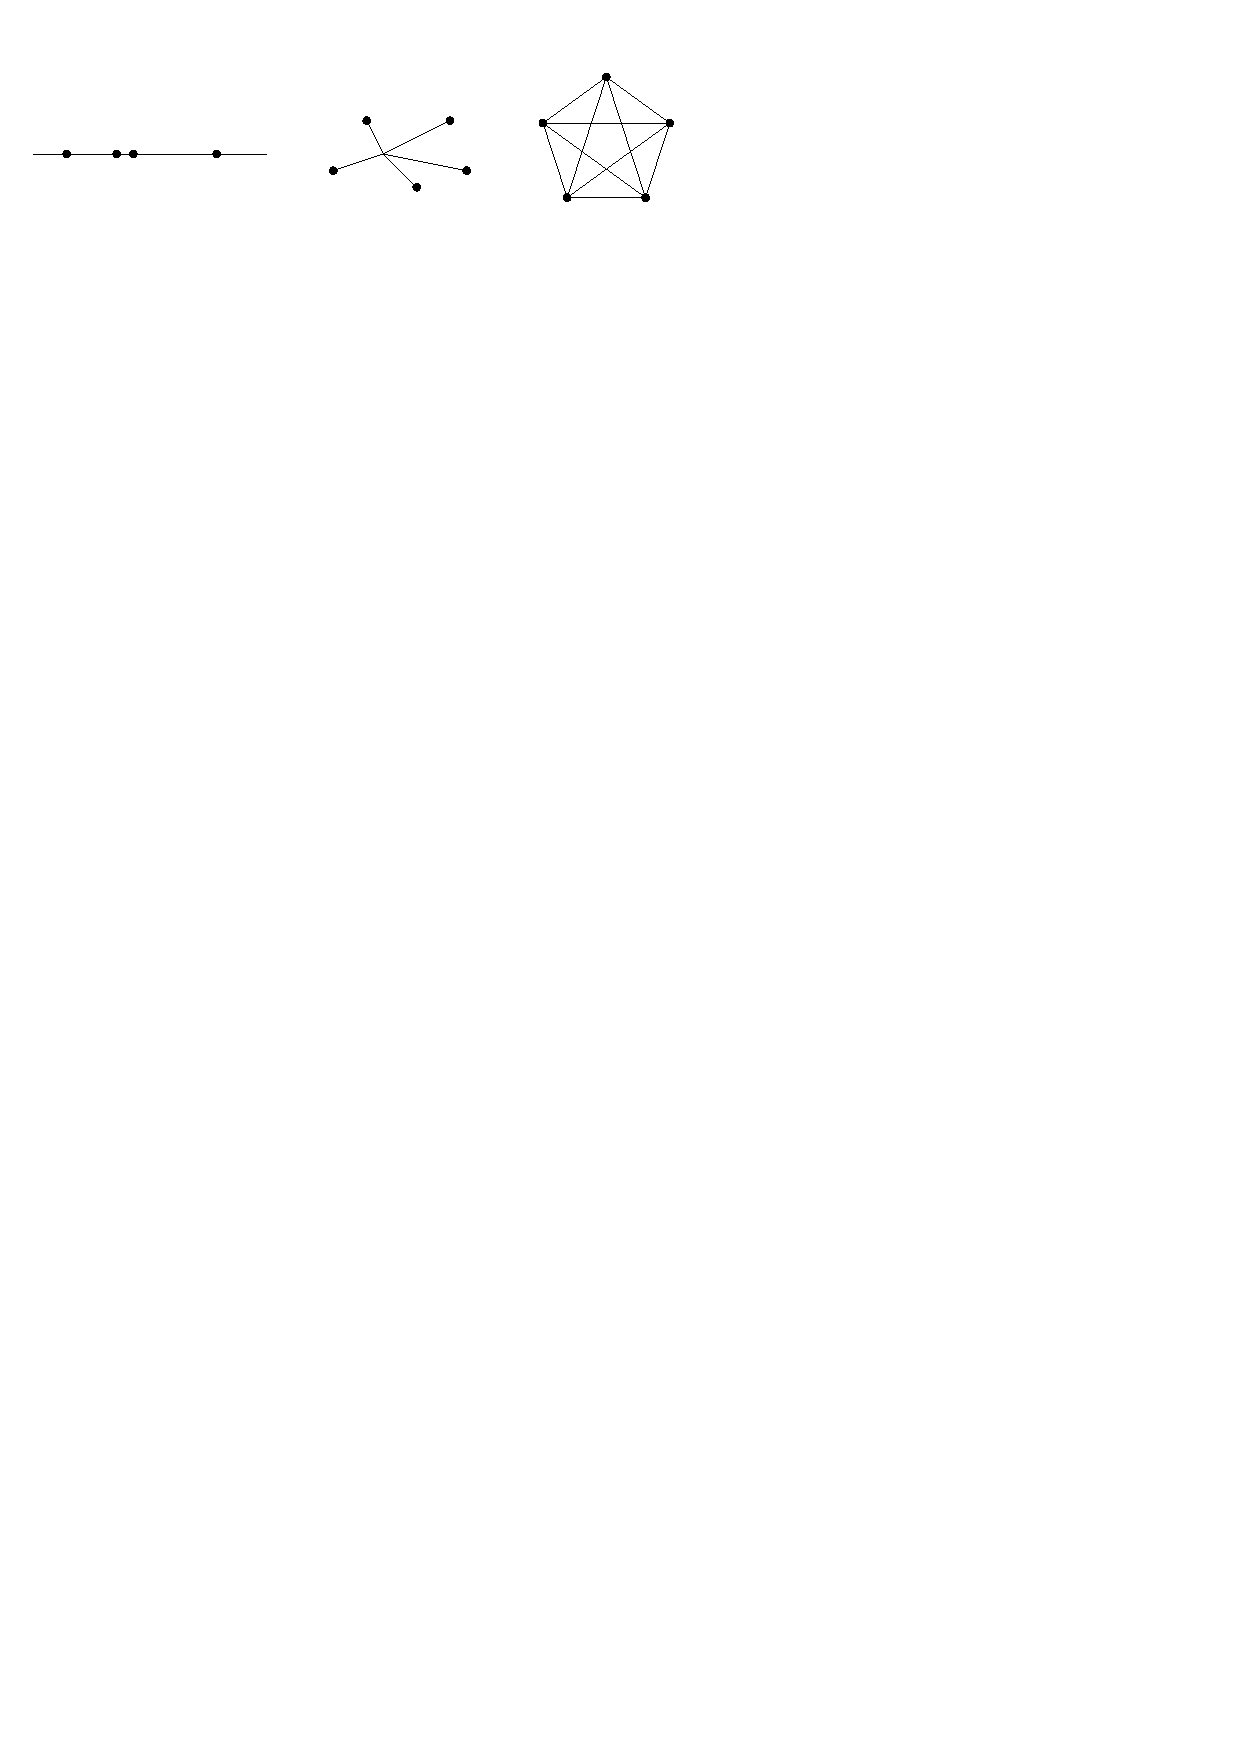
\includegraphics[scale=1.0]{\figdir/graph_classes.pdf}
  \caption{本論文では
    {\graphLine}(左),{\graphStar}(中),{\graphUnit}(右,但し各辺の長さが等しい)を扱う.
    {\graphStar}は葉のみを警邏の対象とする(中央の点は移動の途中で使うのみであり,{\maxIdletime}は定められていない).}
  \label{figure: graph_classes}
\end{figure}
このうち{\graphStar}では
各葉$v$のみに{\maxIdletime}(と中心からの距離$d _v$)が定められている.
つまり厳密には,
警邏の対象となる頂点集合$V$は葉のみであり,
その二点$u$,$v \in V$間の距離が
和$d _u + d _v$の形で表されるという性質を満す完全グラフと考えてよいのであるが(図\ref{figure: stars}),
\begin{figure}
  \centering
  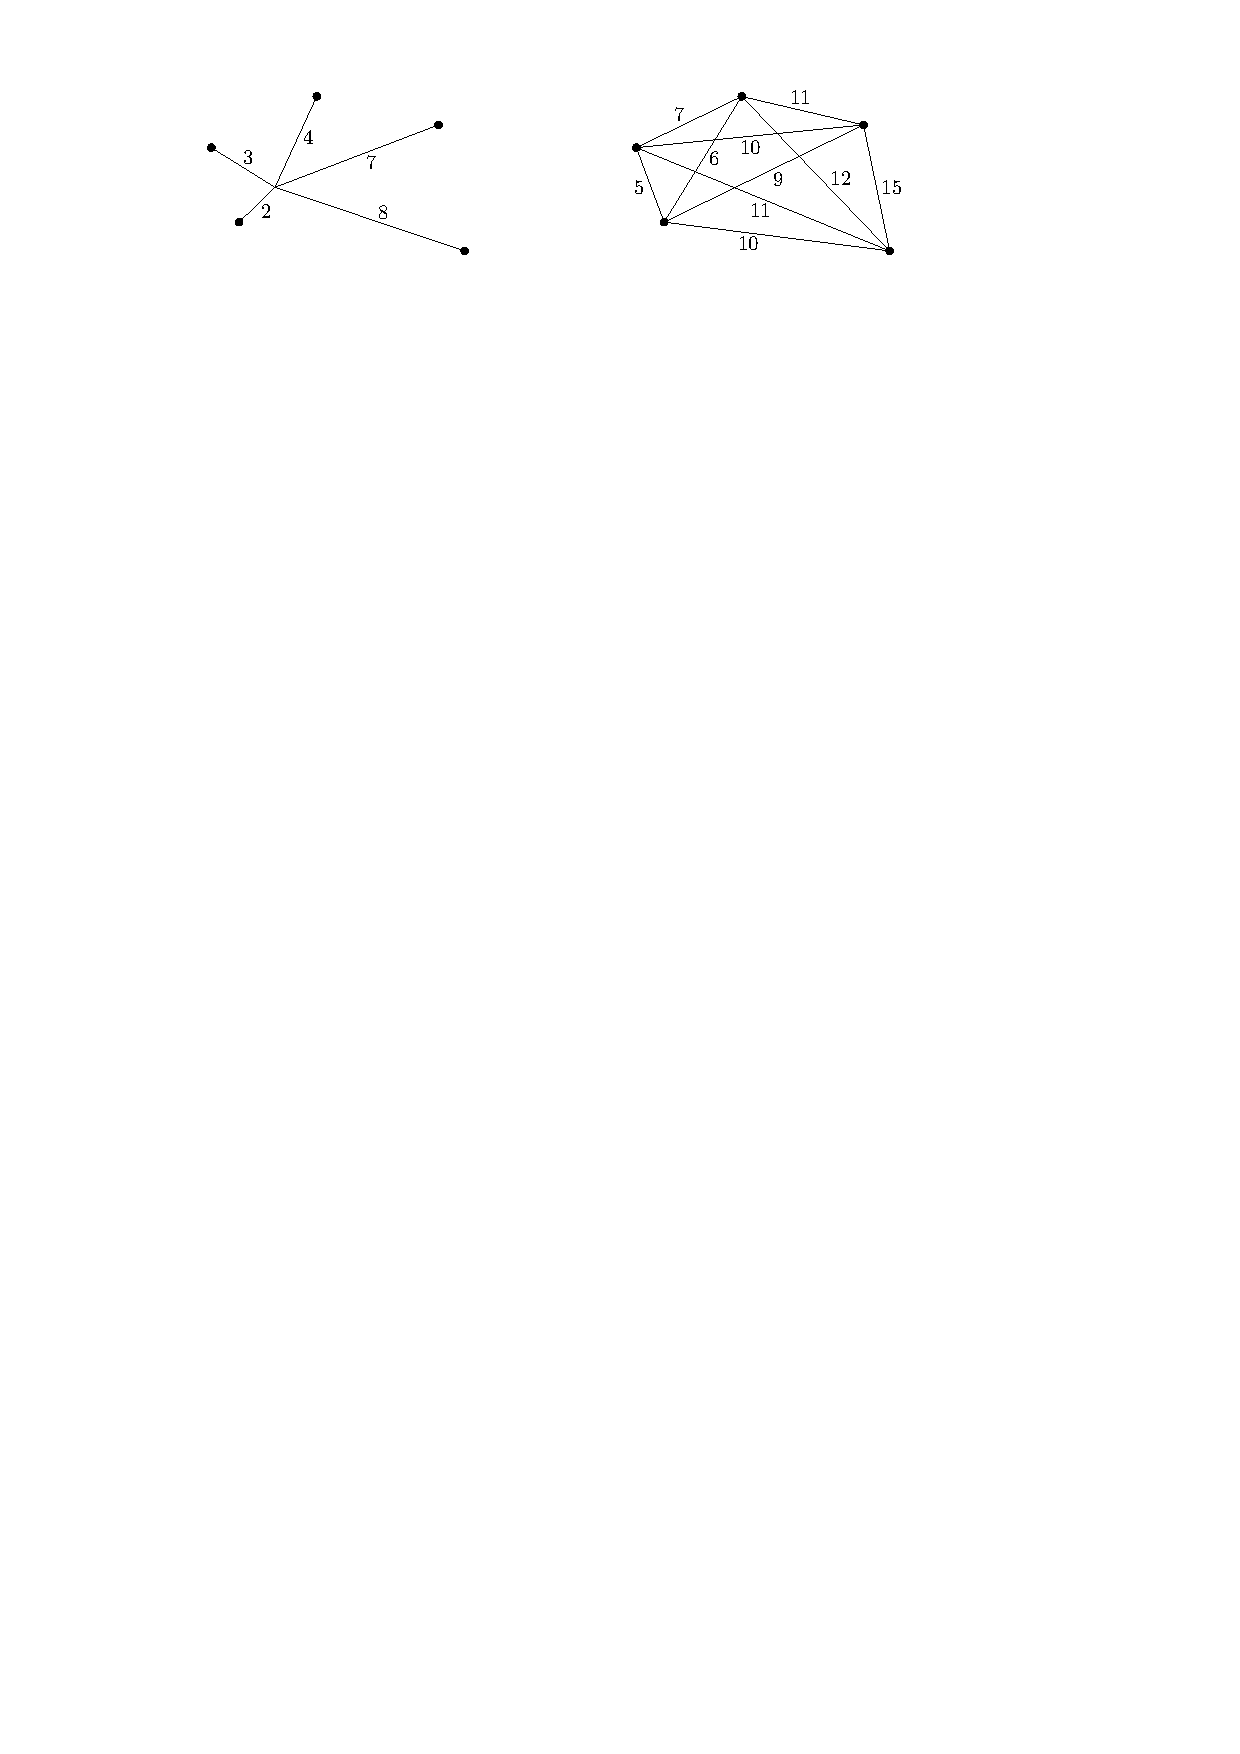
\includegraphics[scale=1.0]{\figdir/stars.pdf}
  \caption{左図の{\graphStar}は,各二点間に右図のような距離を定める.}
  \label{figure: stars}
\end{figure}
以下では便宜上図\ref{figure: graph_classes}や図\ref{figure: stars}左のような形状で図示・説明を行う.
こう考えると各辺の長さが$d$の{\graphUnit}は,
中心から各頂点への距離が$d/2$の{\graphStar}と同じであるから,
{\graphUnit}は{\graphStar}の特殊な場合である.

{\patProb}についての我々の結果を
Coeneらの{\independentPatProb}についての結果との比較も含めて
地図の形ごとにまとめると次のようになる.
それぞれ\ref{chapter: line},\ref{chapter: star},\ref{chapter: unit}章で述べる.
\begin{itemize}
\item 
  {\graphLine}の
  {\independentPatProb}は動的計画法により多項式時間で解けることが
  示されていた\cite[Theorem~11]{coene2011charlemagne}が,
  その正しさは単独警邏という設定に強く依存している.
  本稿では{\patProb}について,
  全点の{\maxIdletime}が等しい場合には多項式時間で解けることを示す
  (定理\ref{theo:LineUnaryIdletimePolyTimeSolvable}).
\item
  {\graphStar}については,
  全点の利得と{\maxIdletime}が等しい場合に限っても,
  {\independentPatProb}はNP困難であることが示されていた\cite[Theorem~10]{coene2011charlemagne}.
  本稿では,この場合の{\patProb}は多項式時間で解けるという興味深い結果を得る
  (定理\ref{theo:StarUnaryProfitAndIdletime}).
  なお利得または{\maxIdletime}を一般にすると,
  巡査が一人であっても(したがって独立かどうかによらず)
  NP困難であることがわかっている\cite[Theorems 5 and 6]{coene2011charlemagne}.
\item 
  {\graphUnit}については,
  本稿では全点の{\maxIdletime}が等しい場合は{\patProb}が多項式時間で解けることを示す
  (定理\ref{theo:UnitUnaryIdletime}).
  地図が{\graphStar}の場合は全点の{\maxIdletime}が等しくても利得が一般だとNP困難になるので,
  これにより{\graphUnit}は{\graphStar}よりも簡単に解ける場合となっていることが分かる.
\end{itemize}

{\graphLine}や{\graphUnit}については,
全点の{\maxIdletime}が等しい場合には上述のように多項式時間で解けるが,
{\maxIdletime}が一般の場合には多項式時間アルゴリズムを見つけることができなかった.
{\graphStar}の{\patProb}は上述の通りNP困難なので\cite[Theorems 5 and 6]{coene2011charlemagne},
{\graphLine}や{\graphUnit}についても
NP困難ではないかと予想したが,これも示すことができなかった.
これらの未解決な場合については,
警邏ではなく定時訪問を目指す次のような問題を考えた.
%
運行$A = (a _1, \ldots, a _m)$が点$v \in U$を
{\exactTime}$(q, r)\ (q \in \Nset, r \in \{ 0, 1, \ldots, q - 1 \})$%
に\defword{定時訪問}するとは,
任意の時刻$t := q k + r\ (k \in \Zset)$に対し
巡査$i$が存在し$a _i (t) = v$であることをいう.

\begin{timeSpecifiedPatrollingProblem}
  巡査の人数$m$と地図$(U, V)$および$V$の各点の{\exactTime}と利得が与えられる.
  $m$人の巡査により全点を定時訪問可能な$V$の部分集合のうち
  利得の和が最大となるものを求めよ.
\end{timeSpecifiedPatrollingProblem}

また,利得最大化ではなく全点を定時訪問可能か判定する問題を{\timeSpecifiedPatProbDecision}と呼ぶ.


{\graphLine}については{\timeSpecifiedPatProbDecision}を解く貪欲アルゴリズムを
\ref{section:LineArbitraryIdletime}節で示す.
{\graphUnit}については{\timeSpecifiedPatProb}がNP困難であることを示す(定理\ref{theo:UnitExacIdletimeNPhard}).


本論文は,
2017年電子情報通信学会総合大会\cite{ieice}%
及び
Japan Conference on Discrete and Computational Geometry, Graphs, and Games 2017\cite{jcdcggg}%
で発表した内容を含む.
